\chapter{Fundamentos del lenguaje}

\section{¿Qué es MATLAB?}

MATLAB es un lenguaje de programación de alto nivel y entorno de desarrollo interactivo, utilizado 
para numerosas aplicaciones de carácter técnico y científicas. MATLAB permite realizar adquisición 
y análisis de datos, desarrollo de algoritmos computacionales, creación y simulación de modelos físicos 
y la visualización gráfica de procesos determinados.  Entre los campos de uso de MATLAB se incluyen 
el procesamiento digital de señales,  audio, imágenes y vídeo, sistemas de control, finanzas 
computacionales, biología computacional, redes neuronales, etc.\\

\textit{Características del lenguaje:}

\begin{itemize}
\item Interpretado: Esta característica le convierte en un lenguaje no muy apto para aplicaciones donde la rapidez de ejecución sea crítica, pero esto mismo facilita la depuración de errores y permite un tiempo de desarrollo reducido en comparación a los lenguajes compilados tradicionales como C/C++.

\item Tipado dinámico: No es necesario declarar el tipo de variable a utilizar, MATLAB reconoce de forma automática el tipo de dato con el que trabajará, aunque claro que es posible declarar un tipo de dato de forma explícita utilizando las funciones de conversión adecuadas.

\item Multiplataforma: MATLAB está disponible para las plataformas más comunes: Unix, Windows, GNU/Linux y Mac OS.

\item Multiparadigma: Soporta programación imperativa, funcional y orientada a objetos.
\end{itemize}


\section{Descripción del entorno de desarrollo}

El entorno de MATLAB mostrado en la figura \ref{f1} pertenece a la versión 2012b, si dispone de otra versión 
quizá encontrará cambios significativos en la interfaz, pero los componentes más importantes permanecen invariables.\\

Como puede observarse en la figura \ref{f1}, se distinguen cuatro componentes en el escritorio del entorno MATLAB, 
los cuáles son:\\

\textbf{Command Window}\\

Ventana de comandos interactiva en la cual deberán introducirse las instrucciones de MATLAB, el prompt \texttt{$>>$} 
le indica que está listo para recibir instrucciones.\\

\begin{informacion}{¿Qué es el prompt?}
En la jerga informática, se denomina prompt al símbolo o caracter que aparece 
en una terminal o consola, cuando esta se encuentra en disposición de aceptar un comando de entrada.
\end{informacion}

\textbf{Current Folder}\\

Carpeta en la que se está situado, y en la que MATLAB buscará y guardará (por defecto) los archivos 
generados durante la sesión.\\

\textbf{Workspace}\\

Ventana que muestra las variables creadas por el usuario durante la sesión, indicando el nombre, valor 
y tipo de la misma.\\

\textbf{Command History}\\

Permite buscar comandos introducidos con anterioridad en la ventana de comandos y ejecutarlos nuevamente 
o copiarlos.\\

\begin{center}
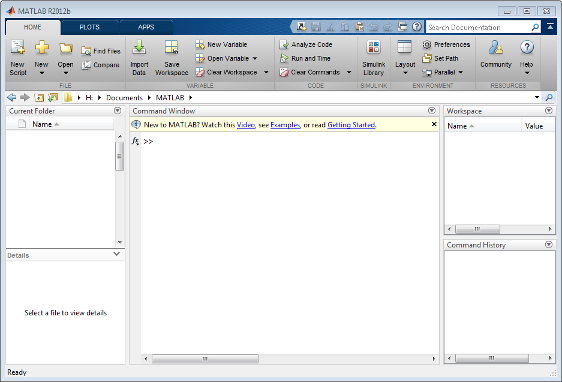
\includegraphics[scale=0.8]{src/ch1/img_1_1.png}
\captionof{figure}{Interfaz de MATLAB R2012b}
\label{f1}
\end{center}

\section{Comandos básicos y generalidades}

\subsection{Consultar ayuda de MATLAB}

Uno de los puntos fuertes de MATLAB es la extensa documentación que viene adjunta al software, la cual 
contiene múltiples ejemplos y recomendaciones para la mayoría de las funciones. Puede acceder a la ayuda 
ubicando el ícono característico de ayuda, o bien tecleando la instrucción doc en la línea de comandos.\\

Si requiere una referencia rápida acerca de un comando o función puede utilizar el comando \texttt{help} 
seguido por el nombre la función a consultar, lo anterior le mostrará en la ventana de comandos una descripción 
breve referente a la función consultada, por ejemplo la siguiente línea le permite consultar ayuda 
rápida acerca del  comando \texttt{clc}:

\begin{verbatim}
>> help clc
	clc    Clear command window.
	clc clears the command window and homes the cursor.
	See also home.
	Reference page in Help browser
	doc clc
\end{verbatim}

\subsection{Limpiar ventana de comandos y variables del workspace}

Generalmente se considera una buena práctica de programación en MATLAB iniciar los programas con 
instrucciones de limpiar la consola (Command Window) y borrar las variables de la memoria. Lo anterior 
se logra utilizando las instrucciones \texttt{clc} para limpiar la ventana de comandos y \texttt{clear} 
para borrar las variables del workspace. Suele acompañarse a la instrucción \texttt{clear} con el argumento 
adicional \texttt{all}, que permite borrar incluso variables globales, es decir 
conjuntamente: \texttt{clear all.}

\subsection{Líneas de comentarios}

Los comentarios de una sola línea en MATLAB deben comenzar  con el símbolo de porcentaje \%, todo 
aquello escrito después de este símbolo será ignorado por el intérprete y reconocido como comentario, 
asignándosele un color verde característico de forma automática.

\begin{verbatim}
% Esto es un comentario en MATLAB
\end{verbatim}

Para hacer bloques de comentarios MATLAB dispone de una sintaxis específica que se muestra enseguida:

\begin{verbatim}
	%{
	Esto es un comentario de múltiples
	líneas en MATLAB, delimitado por 
	llaves conjuntas con el signo % 
	%}
\end{verbatim}

\subsection{Valores especiales}

En la siguiente tabla se resumen algunos valores especiales devueltos por funciones predefinidas en MATLAB:

\begin{table}[h!]
\centering
{\rowcolors{1}{}{gray!20}
\begin{tabular}{p{3cm} p{12cm}} \hline
\rowcolor{header_table_color} \Centering\bfseries Función & \Centering\bfseries Descripción \\
\texttt{ans} & Guarda el ultimo valor no asignado a una variable \\
\texttt{eps} & Tolerancia que MATLAB soporta en los cálculos \\
\texttt{intmax} & Máximo valor entero que puede utilizarse \\
\texttt{intmin} & Mínimo valor entero que puede utilizarse \\
\texttt{realmax}  & Valor de coma flotante máximo que puede representarse \\
\texttt{realmin} & Valor de coma flotante mínimo que puede representarse \\
\texttt{pi} & Constante matemática (3.14159265…) \\
\texttt{inf} & Valor asignado a un número demasiado grande respecto a la
capacidad de cálculo del software. \\
\texttt{NaN} & Iniciales de “Not a Number”, tal cual traducción literal hace
referencia a un valor numérico inválido. \\
\texttt{computer} & Devuelve el tipo de computadora que se está utilizando\\
\texttt{version} & Devuelve la versión de MATLAB \\
\hline
\end{tabular}
\caption{Valores especiales}
\end{table}

\section{Tipos de datos y operadores}

Los tipos de datos más comunes en MATLAB son los siguientes:

\begin{itemize}
\item logical  (tipo booleano o lógico)
\item char (cadenas de caracteres)
\item numeric (datos tipo numérico)
\begin{itemize}
   \item int8, int16, int32, int64 (tipos entero)
   \item uint8, uint16, uint32, uint64  (enteros sin signo)
   \item single (flotantes de precisión simple)
   \item double  (flotantes de precisión doble)
\end{itemize}
\item cell (arreglos de celdas)
\item struct (estructuras)
\end{itemize}

\subsection{Tipo logical}

Las variables de tipo lógico permiten, evidentemente, dos valores, que pueden ser true o false (1 y 0 lógicos).
Una forma de declarar una variable de tipo lógico sería:

\begin{verbatim}
	>> a = true
	a =
	     1
\end{verbatim}
	     
Otra manera que resulta en lo mismo es la siguiente:

\begin{verbatim}
	>> a=logical(1)
	a =
	     1
\end{verbatim}

Las líneas anteriores crean una variable \texttt{a} de tipo lógico con un valor true (1 lógico).


\subsection{Tipo char}

Son cadenas de caracteres, que pueden contener valores alfanuméricos e incluso símbolos especiales. 
Para declararlas no hace falta especificar que son variables tipo char, dado que MATLAB es de tipado 
dinámico y reconoce como tal aquellas cuyo valor asignado se encuentre delimitado por comillas simples, 
un ejemplo muy clásico es el siguiente:

\begin{verbatim}
	>> txt = 'Hola Mundo'
	txt =
	Hola Mundo
\end{verbatim}


\subsection{Tipo numeric}

Normalmente cuando en MATLAB tecleamos un valor numérico o bien lo asignamos a una determinada variable, 
esta será de tipo double, a menos que se haga una conversión explicita a otro tipo de dato. Por ejemplo, 
si insertamos en MATLAB lo siguiente:

\begin{verbatim}
	>> num = 10
	num =
	    10
\end{verbatim}

Y posteriormente tecleamos la instrucción `whos` para verificar el tipo o clase de dicha variable:

\begin{verbatim}
	>> whos
	  Name      Size            Bytes  Class     Attributes
	  num       1x1                 8  double   
\end{verbatim}

Si se requiere utilizar un dato de tipo entero habrá de realizarse la conversión como sigue:

\begin{verbatim}
	>> numInt = int8(23)
	numInt =
	   23
	>> whos
	  Name        Size            Bytes  Class    Attributes
	  numInt      1x1                 1  int8               
\end{verbatim}

\subsection{Tipo cell}

Un cell array es un tipo de dato característico del lenguaje MATLAB que consiste en un arreglo 
multidimensional de celdas que pueden contener cualquier tipo de dato, inclusive otro cell array. 
Un ejemplo muy sencillo de cell array se muestra enseguida:

\begin{verbatim}
	>> C={10,'MATLAB','5',[1 1]}
	C = 
	    [10]    'MATLAB'    '5'    [1x2 double]
\end{verbatim}

\subsection{Tipo struct}

Las estructuras son arreglos de datos que, de forma similar a los cell arrays, pueden almacenar 
variables de diversos tipos. Para la organización de los datos se utilizan campos que pueden 
contener sólo un tipo de dato. A continuación se muestra un ejemplo de cómo crear una estructura:

\begin{verbatim}
	>> Alumno.Nombre='Jorge';
	>> Alumno.Apellido='De Los Santos';
	>> Alumno.Cursos={'Programación','Cálculo','Métodos Numéricos'};
	>> Alumno.Notas=[10 9 10];
	>> Alumno
	Alumno = 
	      Nombre: 'Jorge'
	    Apellido: 'De Los Santos'
	      Cursos: {'Programación'  'Cálculo'  'Métodos Numéricos'}
	       Notas: [10 9 10]
\end{verbatim}


En el capítulo 3 se tratan con más detenimiento las estructuras y su utilidad en la programación en MATLAB.


\subsection{Referencias de función (function handle)}

Las function handle son referencias asociadas a una función nativa de MATLAB o bien a una función 
anónima creada por el usuario.\\

El siguiente ejemplo muestra la creación de una función anónima y su posterior uso mediante su referencia:

\begin{verbatim}
	>> f=@(x) x+cos(x)
	f = 
	    @(x)x+cos(x)
	>> whos
	  Name      Size            Bytes  Class              Attributes
	  f         1x1                32  function_handle              
	>> fzero(f,0) % Raíz de la función 
	ans =
	   -0.7391
	>> f(pi/2) % Evaluando función en un punto
	ans =
	    1.5708
\end{verbatim}


\subsection{Identificar tipos de datos}

Para identificar tipos de datos en MATLAB se cuentan con diversos comandos que nos facilitan esta tarea. 
El comando whos nos proporciona información acerca de las variables existentes en el workspace, tales 
como el nombre, tamaño y tipo. A manera de ejemplo crearemos las siguientes variables e introducimos la 
instrucción whos para verificar el tipo de información que nos imprime en la consola:

\begin{verbatim}
 	>> n=10;
	>> val=false;
	>> s='MATLAB';
	>> C={1,2,3};
	>> ST.Nombre='Anna';
	>> whos
	  Name      Size            Bytes  Class      Attributes
	  C         1x3               360  cell                 
	  ST        1x1               184  struct               
	  n         1x1                 8  double               
	  s         1x6                12  char                 
	  val       1x1                 1  logical      
 \end{verbatim} 


Además del comando \texttt{whos}, puede utilizarse la función \texttt{class} para determinar el tipo de dato de una 
variable pasada como argumento, por ejemplo:

\begin{verbatim}
	>> a=3;
	>> class(a)
	ans =
	double
\end{verbatim}

\subsection{Conversiones entre tipos de datos}

Las conversiones entre tipos de datos son muy utilizadas en la programación en cualquier lenguaje, 
puesto que permiten controlar la precisión de los cálculos, mejorar la presentación de los datos o 
bien evitar errores en la ejecución.

\subsubsection{Entre tipos numéricos}

Cuando se crea una variable de tipo numérico en MATLAB por defecto será de tipo double, por ejemplo, 
creamos una variable llamada num:

\begin{verbatim}
	>> num=2;
	>> class(num)
	ans =
	double
\end{verbatim}

Las conversiones entre tipos numéricos son de sintaxis muy sencilla, solo habrá que especificar el 
tipo de dato al cual se convertirá, siendo permitidos los especificados en la tabla siguiente:\\

\begin{table}[h!]
\centering
{\rowcolors{1}{}{gray!20}
\begin{tabular}{p{5cm} p{5cm} p{5cm}}
\rowcolor{header_table_color} \Centering\bfseries Tipo de dato & \Centering\bfseries Sintaxis de conversión & 
\Centering\bfseries Rango \\
Precisión doble & double(num) & 2.2251e-308 a 1.7977e+308 \\
Precisión simple & single(num) & 1.1755e-38 a 3.4028e+38 \\
Entero de 8 bits & int8(num) & -128 a 127 \\
Entero de 16 bits & int16(num) & -32768 a 32767 \\
Entero de 32 bits & int32(num) & -231 a 231-1 \\
Entero de 64 bits & int64(num) & -263 a 263-1 \\
Entero sin signo de 8 bits & uint8(num) & 0 a 255 \\
Entero sin signo de 16 bits & uint16(num) & 0 a 65535 \\
Entero sin signo de 32 bits & uint32(num) & 0 a 4294967295 \\
Entero sin signo de 64 bits & uint64(num) & 0 a 18446744073709551615 \\
\end{tabular}
\caption{Conversiones entre tipos numéricos}
\end{table}

Así, podemos convertir la variable num, creada con anterioridad, a otro tipo de dato numérico, por 
ejemplo a un entero de 8 bits:

\begin{verbatim}
	>> num=int8(num);
	>> class(num)
	ans =
	int8
\end{verbatim}

Es necesario poner especial atención en los rangos que pueden manipularse con cada tipo numérico, 
debido a que por ejemplo si se realiza la siguiente conversión:

\begin{verbatim}
	>> num=int8(653)
	num =
	  127
\end{verbatim}

El valor que ha sido pasado como argumento de conversión excede el rango para un entero de 8 bits, 
por lo cual simplemente se le asigna el máximo valor permitido para una variable de este tipo.\\

Si requiere verificar por usted mismo los valores máximos y mínimos permitidos para cada tipo de dato, 
puede usar las funciones \texttt{realmin} y \texttt{realmax} para los tipos de coma flotante, y las 
correspondientes \texttt{intmin} e \texttt{intmax} para tipos enteros.

\subsubsection{De string a tipo numérico}

Para este tipo de conversiones MATLAB dispone de la funciones \texttt{str2double} y \texttt{str2num}, 
en algunos casos no notará la diferencia en los resultados, salvo en la rapidez de ejecución. Pese a lo 
anterior, es necesario tomar en cuenta cómo trabaja cada función y cual le resulta de utilidad; 
con \texttt{str2double} se convierte una variable tipo string en un valor de tipo double, 
la función \texttt{str2num} también realiza conversión a tipo double pero además realiza conversiones 
a otros tipos de datos numéricos si se especifica de manera explícita, de hecho esta tiene una 
funcionalidad muy similar a la de la función \texttt{eval}. Los siguientes ejemplos muestran las 
diferencias y utilidades de las funciones descritas.


\begin{verbatim}
	>> a=str2double('1237')
	a =
	        1237
	>> b=str2num('1237')
	b =
	        1237
	>> whos
	  Name      Size            Bytes  Class     Attributes
	  a         1x1                 8  double              
	  b         1x1                 8  double     
\end{verbatim}


\subsection{Operadores aritméticos, relacionales y lógicos}

En la siguiente tabla se resumen los operadores más importantes en MATLAB.

\begin{table}[h!]
\centering
{\rowcolors{1}{}{gray!20}
\begin{tabular}{p{3cm} p{9cm}}
\rowcolor{header_table_color} \Centering\bfseries Operador  & \Centering\bfseries Descripción \\
\multicolumn{2}{c}{\bfseries Operadores aritméticos} \\
+ & Operador  suma \\
- & Operador resta \\
* & Operador multiplicación (escalares) \\
/ & Operador división \\
./ & División elemento a elemento (matrices) \\
.* & Multiplicación elemento a elemento (matrices) \\
\multicolumn{2}{c}{\bfseries Operadores lógicos} \\
\& & Operador lógico and \\
$|$ & Operador lógico or \\
$\sim$ & Operador lógico not \\
\multicolumn{2}{c}{\bfseries Operadores relacionales} \\
== & Igual a  \\
$<$ & Menor que \\
$>$ & Mayor que \\
$<$= & Menor o igual que \\
$>$= & Mayor o igual que \\
$\sim =$ & Diferente de \\
\end{tabular}
\caption{Conversiones entre tipos numéricos}
\end{table}


\section{Un mini tutorial de introducción}

Una vez conocidos los tipos de datos y los operadores, podemos comenzar con una breve introducción 
al uso de MATLAB como una poderosa calculadora muy fácil de utilizar.\\

Como se ha descrito en secciones anteriores, el command window o ventana de comandos es la parte 
del entorno MATLAB que nos permite interactuar de forma dinámica, si tecleamos una instrucción 
automáticamente nos devolverá un resultado y se crearán variables en las cuales se almacenen 
los diversos valores de salida. Por ejemplo, vamos a teclear una simple suma aritmética:

\begin{verbatim}
	>> 3+2
	ans =
	     5
\end{verbatim}

Puede verificar que en el workspace ahora aparece una variable llamada \texttt{ans} con valor de 5, 
en \texttt{ans} se guarda por defecto el último resultado no asignado a una variable, podríamos asignar 
el resultado de la suma a una variable específica:

\begin{verbatim}
	>> suma=3+2
	suma =
	     5
\end{verbatim}

Podemos también asignar valores a determinadas variables y enseguida utilizarlas para ejecutar 
alguna operación, por ejemplo:

\begin{verbatim}
	>> a=5;
	>> b=7;
	>> a*b
	ans =
	    35
	>> a-b
	ans =
	    -2
	>> a/b
	ans =
	    0.7143
\end{verbatim}

Note que el colocar un punto y coma (;) al final de una instrucción evita que se muestre un resultado de salida, 
lo cual no afecta en el almacenamiento de los valores correspondientes, pero podría resultar de mucha ayuda al 
momento de seleccionar los valores que se quieren mostrar en la ventana de comandos.\\

MATLAB también tiene disponible diversas funciones matemáticas predefinidas, que pueden ser aplicadas 
sobre un número o sobre una matriz o arreglo de números. Algunas funciones trigonométricas:

\begin{verbatim}
	>> sin(pi/2)
	ans =
	     1
	>> cos(pi/4)
	ans =
	    0.7071
	>> tan(pi/3)
	ans =
	    1.7321
\end{verbatim}

Note que el valor de la constante $\pi$ está predefinida en MATLAB mediante la cadena \texttt{pi}:

\begin{verbatim}
>> pi
ans =
    3.1416
\end{verbatim}

MATLAB devuelve un valor de 3.1416, lo cual es un valor \textit{redondeado} de $\pi$, pero esto 
es cuestión solamente de la representación, normalmente se utiliza el formato short (4 dígitos después
del punto decimal) para la representación de valores numéricos, internamente MATLAB utiliza más 
digitos para \textit{manejar} y operar con el valor de $\pi$. Si queremos obtener más digitos en 
la salida por consola podemos cambiar el formato de salida:

\begin{verbatim}
>> format long
>> pi
ans =
   3.141592653589793
\end{verbatim}

El formato largo permite representar una cantidad con 16 decimales. Incluso es posible \textit{forzar} 
a que se muestre una representación en forma racional:

\begin{verbatim}
>> format rat
>> pi
ans =
     355/113   
>> 0.1+0.123
ans =
     223/1000  
>> 0.125
ans =
       1/8
\end{verbatim}

Se puede crear una lista o arreglo de valores numéricos encerrando estos entre corchetes, 
y separando cada elemento por comas o espacios.

\begin{verbatim}
>> A=[5,8,10,2,7]
A =
     5     8    10     2     7
>> B=[3 7 1 0 -2]
B =
     3     7     1     0    -2
\end{verbatim}

Se puede obtener el valor máximo y mínimo de un arreglo numérico utilizando las funciones \texttt{max} y 
\texttt{min} respectivamente.

\begin{verbatim}
>> max(A)
ans =
    10
>> min(A)
ans =
     2
\end{verbatim}

También podemos calcular el promedio de los valores utilizando la función \texttt{mean}:

\begin{verbatim}
>> mean(A)
ans =
    6.4000
\end{verbatim}

Obtener la cantidad de elementos que componen lista con \texttt{length} o \texttt{numel}:

\begin{verbatim}
>> length(A)
ans =
     5
>> numel(A)
ans =
     5
\end{verbatim}


\section{Ficheros de comandos}

Los ficheros de comandos, conocidos también como \textit{scripts}, son archivos de texto sin formato 
(ASCII) con la extensión característica de los archivos de MATLAB (*.m), se utilizan para 
almacenar una serie de comandos o instrucciones que se ejecutan sucesivamente y que habrán 
de realizar una tarea específica. Los scripts de MATLAB pueden editarse utilizando cualquier 
editor de texto sin formato (Bloc de Notas, Notepad++, Sublime Text, etc…), aunque es más 
recomendable utilizar el editor de MATLAB, puesto que proporciona herramientas que facilitan 
la corrección de errores, el control sobre la ejecución del código y la capacidad de 
autocompletado y sugerencias cuando se utilizan funciones nativas de MATLAB.\\

Para crear un nuevo script puede pulsar la combinación \textbf{Ctrl + N} (bajo SO Windows), o buscar 
en la interfaz de MATLAB la opción New y enseguida seleccionar Script; si prefiere hacerlo 
desde la ventana de comandos puede introducir el comando edit que le abrirá un nuevo script.\\

Para guardar un fichero de comandos utilice la opción \textbf{Save} de la barra de herramientas  o 
bien mediante la combinación de teclas \textbf{Ctrl + S} en Windows. Debe tomarse en cuenta que 
al guardar un script se le proporcione un nombre que no entre en conflicto con las funciones 
nativas de MATLAB o las palabras reservadas del lenguaje. Algunas recomendaciones que deben 
seguirse para nombrar un script son:

\begin{itemize}
\item El nombre deberá contener sólo letras, números o guiones bajos.
\item No deberá comenzar con un carácter diferente a una letra (Por ejemplo: 102metodo.m, es un nombre inválido dado que comienza con un número).
\item Evite utilizar nombres de funciones nativas de MATLAB o palabras reservadas del lenguaje que podrían ocasionar conflictos.
\end{itemize}






\section{Entradas y salidas en el Command Window}

En la sección 1.2 se describió al Command Window (ventana de comandos) y se hizo referencia a este 
como la parte del escritorio de MATLAB que permite interactuar tecleando instrucciones y 
devolviendo al instante un resultado. En esta sección veremos cómo utilizar funciones que 
permitan introducir y mostrar ciertos valores de manera controlada por el usuario.

\subsection{La función input}

La función input permite \textit{pedir} un valor al usuario utilizando una cadena de caracteres 
como prompt, la sintaxis es muy sencilla:

\begin{verbatim}
	var=input('Introduzca un valor: ');
\end{verbatim}

En la variable var se guarda el valor que el usuario introduzca, los valores aceptados por 
la función input pueden ser de tipo numérico, cell arrays, e inclusive tipo char. Aunque 
para introducir cadenas de texto la función input dispone de un modificador que hará que 
la entrada se evalúe como una variable tipo char o cadena de texto, la sintaxis para 
esto es la siguiente:

\begin{verbatim}
	var=input('Introduzca una cadena de texto: ', 's');
\end{verbatim}

La letra s entre comillas simples le indica a MATLAB que deberá evaluar la entrada como tipo string.

\subsection{Salida sin formato: la función disp}

La función disp muestra en pantalla el valor de una determinada variable que se pasa como 
argumento, por ejemplo:

\begin{verbatim}
	>> a=3;
	>> disp(a)
	     3
\end{verbatim}

Para el caso anterior se pasa como argumento la variable a que ha sido declarada previamente 
y simplemente se muestra el valor correspondiente a esta. Las variables a mostrar pueden ser 
de cualquier tipo, incluyendo cadenas de texto, matrices, cell arrays y estructuras, 
véanse los siguientes ejemplos:

\begin{verbatim}
	>> disp(magic(3))
	     8     1     6
	     3     5     7
	     4     9     2
	>> disp({1,0,2,-2})
	    [1]    [0]    [2]    [-2]
	>> disp('Hola Mundo')
	Hola Mundo
\end{verbatim}

Con disp también es posible mostrar enlaces a un sitio web, utilizando la sintaxis HTML para 
un enlace dentro de la función disp, por ejemplo:

\begin{verbatim}
	>> disp('<a href="http://matlab-typ.blogspot.mx">MATLAB TYP</a>');
	MATLAB TYP
\end{verbatim}

\subsection{La función fprintf}

Con fprintf es posible dar formato a la salida que se quiere imprimir en pantalla, por ejemplo, es posible
especificar el número de decimales que se mostrarán o bien si se quiere mostrar como un entero o quizá
como una cadena de texto. La sintaxis de la función fprintf es como sigue:

\begin{verbatim}
fprintf('Especificaciones de formato',a1,...,an);
\end{verbatim}

Donde las especificaciones de formato incluyen uno o más de los identificadores de un mismo tipo o
combinados que se muestran en la siguiente tabla:

\begin{table}[h!]
\centering
{\rowcolors{1}{}{gray!20}
\begin{tabular}{p{4cm} p{7cm}} \hline
\rowcolor{header_table_color} \Centering\bfseries Identificador & \Centering\bfseries Formato de salida \\
\texttt{\%d} & Tipo entero \\
\texttt{\%f} & Tipo coma flotante \\
\texttt{\%g} & Tipo coma flotante compacta. \\
\texttt{\%u} & Tipo entero sin signo \\
\texttt{\%e} & Tipo coma flotante, notación exponencial \\
\texttt{\%s} & Tipo char, cadena de texto \\
\texttt{\%c} & Tipo char, carácter a carácter.\\
\hline
\end{tabular}
\caption{Opciones de formato para \texttt{fprintf}}
\end{table}

Véase el siguiente ejemplo:

\begin{verbatim}
>> fprintf('%d',pi);
3.141593e+00>>
\end{verbatim}

Observe que se imprime el valor de $\pi$ en este caso, pero el prompt de la ventana de comandos queda situado
justo después del valor de salida en la misma línea, para evitar lo anterior puede utilizar la secuencia de
escape \n después del valor a imprimir, lo cual le indica a MATLAB que debe comenzar en una nueva
línea. Modificamos y vemos el resultado que produce:

\begin{verbatim}
>> fprintf('%d\n',pi);
3.141593e+00
\end{verbatim}

Ahora observe lo que se imprime utilizando otros identificadores:

\begin{verbatim}
>> fprintf('%f\n',pi);
3.141593
>> fprintf('%g\n',pi);
3.14159
>> fprintf('%e\n',pi);
3.141593e+00
>> fprintf('%u\n',pi);
3.141593e+00
\end{verbatim}

Para las salidas de coma flotante puede especificar el número de decimales que tendrá la salida, por ejemplo
si desea mostrar solamente dos decimales del número $\pi$:

\begin{verbatim}
>> fprintf('%.2f\n',pi);
3.14
\end{verbatim}


\section{Funciones}

\subsection{Funciones, una introducción}

Las funciones son porciones de código que por lo general aceptan argumentos o valores de 
entrada y devuelven un valor de salida. Una función es una herramienta muy útil en la 
programación, dado que permite la reutilización de código para procedimientos que así 
lo requieran, así como una facilidad significativa para mantener el código, lo cual se 
traduce en una mayor productividad.  MATLAB, de hecho, está compuesto por una multitud 
de funciones agrupadas en toolboxs, cada una de ellas pensada para resolver una 
situación concreta.\\

La estructura básica de una función contiene los siguientes elementos:

\begin{itemize}
\item La palabra reservada function
\item Los valores de salida
\item El nombre de la función
\item Los argumentos de entrada
\item Cuerpo de la función 
\end{itemize}

Para una mejor comprensión de cada uno de esos elementos, refiérase a las siguientes 
líneas de código:

\begin{verbatim}
	function res = suma(a,b)
	res = a+b;
	end
\end{verbatim}

La función anterior llamada suma, recibe como argumentos de entrada dos valores numéricos 
a y b, y devuelve un resultado guardado en res que equivale a la suma aritmética de las 
variables de entrada. Si ejecutamos la función en la ventana de comandos obtenemos 
algo similar a esto:

\begin{verbatim}
	>> s=suma(3,2)
	s =
	     5
\end{verbatim}

Si no hace una asignación el resultado devuelto se guarda en la variable \texttt{ans}.

\subsection{Verificar argumentos de entrada y salida}

Cuando se crea una función es recomendable verificar si la cantidad de argumentos de 
entrada corresponden a los soportados, o bien, si el tipo de dato que se ha introducido 
es el adecuado para proceder con el resto de la programación; MATLAB proporciona los 
comandos \texttt{nargin} y \texttt{nargout} que sirven para \textit{contar} el número de argumentos de 
entrada y salida respectivamente.\\

Utilizando como ejemplo la función suma creada con anterioridad, podemos verificar que 
el número de argumentos sean exactamente dos para poder proceder y en caso contrario 
enviar al usuario un mensaje de error en la ventana de comandos, el código implicado 
sería similar al siguiente:

\begin{verbatim}
	function res = suma(a,b)
	if nargin==2
	    res=a+b;
	else
	    error('Introduzca dos argumentos de entrada');
	end
	end
\end{verbatim}

Si ejecutamos la función pasándole solamente un argumento de entrada nos devolverá un mensaje de error:

\begin{verbatim}
	>> s=suma(7)
	Error using suma (line 5)
	Introduzca dos argumentos de entrada
\end{verbatim}

\subsection{Sub-funciones}

Las sub-funciones son funciones definidas dentro del espacio de otra función principal. 
Se utilizan como funciones auxiliares con la finalidad de hacer más legible el código y 
facilitar la depuración de errores. Enseguida se muestra el ejemplo de una sub-función:

\begin{verbatim}
	function r=isfibo(num)
	% Determina  si un  número  entero  forma  parte
	% de la sucesión de Fibonacci, devuelve un valor
	% de tipo lógico.
	ff=fibonacci(num);
	if any(ff==num)
	    r=true;
	else
	    r=false;
	end
	    function F=fibonacci(n)
	        F(1:2)=1;
	        i=3;
	        while 1
	            F=[F F(i-1)+F(i-2)];
	            if F(end) >= n,break,end;
	            i=i+1;
	        end
	    end
	end
\end{verbatim}

La función anterior isfibo determina si el entero pasado como argumento de entrada 
pertenece a la sucesión de Fibonacci, para ello utiliza como una función auxiliar a 
la sub-función fibonacci que se encarga de generar la sucesión de Fibonacci en un 
intervalo dado y guardarlo en un vector de salida. Una sub-función puede ser llamada 
solamente por la función principal que la contiene.

\subsection{Argumentos variables}

En la introducción a las funciones se ha mencionado que estas por lo general 
tienen un número específico de argumentos de entrada y salida, no obstante se 
presentan situaciones en donde  los argumentos de entrada o salida de una función 
no son fijos o bien los argumentos pueden ser demasiados de tal modo que resulte 
incómodo definirlos en la línea correspondiente. Para solucionar lo anterior MATLAB 
permite el uso de varargin y varargout como argumentos de entrada y salida 
respectivamente. Para tener una  idea más práctica de lo anterior véase el ejemplo siguiente:

\begin{matlab}
	function m=max2(varargin)
	if nargin==1
	    v=varargin{1};
	    m=v(1);
	    for i=2:length(v)
	        if v(i)>m
	            m=v(i);
	        end
	    end 
	elseif nargin==2
	    a=varargin{1};
	    b=varargin{2};
	    if a>b
	        m=a;
	    else
	        m=b;
	    end
	end
	end
\end{matlab}

La función anterior max2 emula a la función nativa  max, puede recibir como argumento 
de entrada un vector o bien dos valores escalares. Si observa el código anterior notará 
que varargin es un cell array que guarda todos los argumentos de entrada pasados a la 
función, como se verá en el capítulo 3 la manera de acceder a los elementos de un 
cell array es utilizando la sintaxis: var{k}, donde var es la variable en la que está 
almacenada el cell array y k es el k-ésimo elemento contenido en el cell array.

\subsection{Ayuda de una función}

Como parte de las buenas prácticas de programación es recomendable incluir comentarios 
dentro de una función que indiquen el propósito de esta, así como una descripción breve 
de los argumentos de entrada y salida e incluso un ejemplo concreto de la misma.\\

Por convención estos comentarios deben colocarse justamente después de la definición de 
la función y antes de todo el código restante, además de que esto servirá como referencia 
al resto de usuarios también le permitirá a MATLAB interpretarlo como las líneas de ayuda 
cuando se le solicite expresamente mediante la función help. Véase el siguiente ejemplo:

\begin{verbatim}
	function [x1,x2]=ecuad(a,b,c)
	% Resuelve una ecuación cuadrática de la forma:
	% a*x^2+b*x+c=0
	%
	% Argumentos de entrada:
	%          a  -  Coeficiente cuadrático
	%          b  -  Coeficiente lineal
	%          c  -  Coeficiente constante
	%
	% Argumentos de salida:
	%          x1,x2  - Raíces de la ecuación cuadrática 
	%
	% Ejemplo:
	%         >> [r1,r2]=ecuad(-1,2,1);
	%
	 
	x1=(1/(2*a))*(-b+sqrt(b^2-4*a*c));
	x2=(1/(2*a))*(-b-sqrt(b^2-4*a*c));
	end
\end{verbatim}

Podemos teclear help ecuad en la ventana de comandos y verificar lo que MATLAB nos 
devuelve como ayuda de la función:

\begin{verbatim}
	>> help ecuad
	  Resuelve una ecuación cuadrática de la forma:
	  a*x^2+b*x+c=0
	  Argumentos de entrada:
	           a  -  Coeficiente cuadrático
	           b  -  Coeficiente lineal
	           c  -  Coeficiente constante
	  Argumentos de salida:
	           x1,x2  - Raíces de la ecuación cuadrática 
	  Ejemplo:
	          >> [r1,r2]=ecuad(-1,2,1);
\end{verbatim}

Es común agregar a la ayuda de una función algunas referencias hacia otras funciones 
similares, para ello en los comentarios debe agregar una línea que comience con las 
palabras “SEE ALSO” (Ver también), seguidas de las funciones similares separadas por 
comas, véase el ejemplo a continuación:

\begin{verbatim}
	function [x1,x2]=ecuad(a,b,c)
	% Resuelve una ecuación cuadrática de la forma:
	% a*x^2+b*x+c=0
	%
	% Argumentos de entrada:
	%          a  -  Coeficiente cuadrático
	%          b  -  Coeficiente lineal
	%          c  -  Coeficiente constante
	%
	% Argumentos de salida:
	%          x1,x2  - Raíces de la ecuación cuadrática 
	%
	% Ejemplo:
	%         >> [r1,r2]=ecuad(-1,2,1);
	%
	% SEE ALSO roots,solve,fzero
	%
	 
	x1=(1/(2*a))*(-b+sqrt(b^2-4*a*c));
	x2=(1/(2*a))*(-b-sqrt(b^2-4*a*c));
	end
\end{verbatim}

\begin{verbatim}
	>> help ecuad
	  Resuelve una ecuación cuadrática de la forma:
	  a*x^2+b*x+c=0 
	  Argumentos de entrada:
	           a  -  Coeficiente cuadrático
	           b  -  Coeficiente lineal
	           c  -  Coeficiente constante
	  Argumentos de salida:
	           x1,x2  - Raíces de la ecuación cuadrática 
	  Ejemplo:
	          >> [r1,r2]=ecuad(-1,2,1);

	  SEE ALSO roots,solve,fzero
\end{verbatim}

\section{Bifurcaciones y bucles}

\subsection{Sentencia if-elseif-else}

La sentencia if se utiliza  como bifurcación simple por sí sola, es decir, en aquellas 
situaciones en las cuales se requiera evaluar solamente una condición, por ejemplo, 
suponga que tiene dos números a y b y necesita comprobar si son iguales y ejecutar una 
acción, para ello bastaría con una sentencia if simple:

\begin{verbatim}
	if a==b
	    disp('a es igual a b');
	end
\end{verbatim}

A  diferencia del caso anterior hay situaciones que requieren la ejecución de una acción 
cuando la condición se cumpla y de otra en caso contrario, entonces puede utilizarse 
una bifurcación doble formada por las sentencias  if-else. Retomando el ejemplo para 
la bifurcación if simple, podríamos modificarlo de tal manera que envíe también un 
mensaje (ejecute una acción) para cuando la condición no se cumple:

\begin{verbatim}
	if a==b
	    disp('a es igual a b');
	else
	    disp('a es diferente de b');
	end
\end{verbatim}

Ahora imagine que para los ejemplos anteriores  se necesita especificar si  a=b, si a>b 
o bien si a<b, lo cual implicaría tener una sentencia de selección múltiple 
if-elseif-else que permite escoger entre varias opciones, evaluándose en orden 
descendente, por ejemplo refiérase a la siguiente estructura:

\begin{verbatim}
	if cond1
	    % Instrucciones
	elseif cond2 
	    % Instrucciones
	elseif cond3
	    % Instrucciones
	    .
	    .
	    .
	elseif condN
	    % Instrucciones
	else
	    % Instrucciones
	end
\end{verbatim}

MATLAB evalúa primeramente la condición 1 contenida en la sentencia if (cond1) y en 
el caso de no cumplirse evalúa la siguiente condición de forma sucesiva (cond2, cond3, …); 
finalmente y en el caso de que ninguna de las opciones evaluadas se cumpla, se ejecuta 
la instrucción contenida en la sentencia else. A continuación se muestra el ejemplo de 
una bifurcación múltiple para la situación descrita al principio:

\begin{verbatim}
	if a==b
	    disp('a es igual que b');
	elseif a>b
	    disp('a es mayor que b');
	elseif a<b
	    disp('a es menor que b');
	end
\end{verbatim}

\subsection{Sentencia switch}

La sentencia switch es una bifurcación múltiple que permite seleccionar entre varias 
opciones o casos la acción a ejecutar. La sintaxis general es:

\begin{verbatim}
	switch var
	   case opc1
	      % Instrucciones
	   case opc2
	      % Instrucciones
	    .
	    .
	    .
	   otherwise
	      % Intrucciones
	end
\end{verbatim}

Siendo var la variable que servirá como criterio de selección. Después de la palabra 
reservada case, se coloca el valor de var para el cual se ejecutarán esas instrucciones, 
y en otherwise se insertan las instrucciones que MATLAB deberá ejecutar por defecto en 
caso de no cumplirse ninguno de los casos especificados.\\

Enseguida se muestran dos ejemplos correspondientes a la sentencia de selección switch:

\begin{verbatim}
	X=input('Inserte 0 o 1: ');
	switch X
	    case 0
	        disp('Insertó cero');
	    case 1
	        disp('Insertó uno');
	    otherwise
	        warning('Valor incorrecto, verifique');     
	end


	letra=input('Inserte una letra: ','s');
	switch letra
	    case {'a','e','i','o','u'}
	        disp('Es una vocal');
	    otherwise
	        disp('Es una consonante');
	end
\end{verbatim}


\subsection{Bucle for}

La sintaxis general de un bucle for se muestra enseguida:

\begin{verbatim}
	for i=inicio:incremento:fin
	    % Instrucciones...
	end
\end{verbatim}

El valor inicio es a partir del cual se ejecutará el ciclo, el incremento es la 
cantidad que varía en cada paso de ejecución, y el valor de final establece el 
último valor que  tomará el ciclo.\\

El siguiente código muestra un ciclo for muy básico, el cual simplemente muestra 
en consola el valor actual adquirido por la variable.

\begin{verbatim}
	for i=1:10
	    fprintf('Valor actual: %g \n',i);
	end
\end{verbatim}

Cuando no se especifica el incremento, como el caso anterior, MATLAB asume que es unitario.\\

Es posible utilizar ciclos for anidados, por ejemplo para cuando se requiere 
recorrer una matriz en sus dos dimensiones y ejecutar operaciones elemento 
por elemento. Véase el siguiente ejemplo:

\begin{verbatim}
	A=round(rand(5)*10);
	for i=1:5
	    for j=1:5
	        disp(A(i,j));
	    end
	end
\end{verbatim}


\subsection{Bucle while}

El bucle while se utiliza, por lo general, cuando no se tiene un rango definido 
sobre el cual se realice la ejecución del ciclo o bien cuando la terminación del 
mismo viene dada por una condición. La sintaxis más común es:

\begin{verbatim}
	while cond
	    % Instrucciones
	    % ...
	    % ...
	    % ...
	end
\end{verbatim}

Donde \texttt{cond} es la condición que determina la finalización de ejecución.\\

Enseguida se muestra un ejemplo muy básico que muestra en pantalla el valor 
de una variable utilizada como referencia:

\begin{verbatim}
	k=1;
	while k<10
	    disp(k);
	    k=k+1;
	end
\end{verbatim}

Lo anterior muestra en consola el valor de k mientras esta sea menor a 10, es decir 
muestra todos los valores enteros en el intervalo [1  9], es importante notar que 
la variable k debe incrementarse en cada ciclo para que en un momento determinado 
la condición de finalización se cumpla, de lo contrario se convertiría en un bucle infinito.\\

Ahora, veamos un ejemplo más práctico. La aproximación de una raíz cuadrada por 
el método babilónico implica realizar n iteraciones mediante la siguiente expresión:

$$r_n(x) = \frac{1}{2}(\frac{x}{r_{n-1}}+r_{n-1})$$

Donde x es el número del cual se calcula la raíz cuadrada. A continuación se muestra 
el código implementado en MATLAB utilizando un bucle \texttt{while}:

\begin{verbatim}
	x=input('Introduzca un número positivo: ');
	r=x;
	ra=0;
	while ra~=r
	    ra=r;
	    r=(1/2)*(x/r+r);
	end
	fprintf('\nRaíz cuadrada de %g = %g\n\n',x,r);
\end{verbatim}

Como se observa, en la variable ra se guarda la raíz aproximada calculada en una 
iteración anterior, de manera que esta sirva como comparación respecto a la nueva 
raíz calculada, el bucle termina cuando la diferencia entre el valor actual y el 
anterior es inferior a la tolerancia numérica (eps) soportada por MATLAB y por 
ende pasan a considerarse como valores iguales.

\begin{informacion}{El bucle while \& if-break}
Es común utilizar el ciclo while poniendo un valor verdadero como condición, y 
usar la sentencia combinada \texttt{if-break} como punto de parada, por ejemplo:

\begin{verbatim}
while true
    a = randi(10);
    if a>5
        break;
    end
end
\end{verbatim}

\end{informacion}


\section{Fecha y hora}

Primeramente es importante mencionar que MATLAB maneja tres formatos de fechas 
y hora, a saber:

\begin{itemize}
\item Un vector de seis elementos los cuales son: [año, mes, día, hora, minuto, segundo].
\item Un valor escalar de coma flotante (tipo double), en el cual la parte entera representa la cantidad de días que han transcurrido desde el año cero (calendario gregoriano) y la parte decimal representa la fracción del día trascurrido.
\item Una cadena de texto con la forma \texttt{'dd-mmm-aaa HH:MM:SS'}.
\end{itemize}

Para obtener la fecha actual MATLAB proporciona el comando now:

\begin{verbatim}
	>> now
	ans =
	   7.3575e+05
\end{verbatim}

Lo anterior podría resultar útil para efectos de cálculo pero no es tan significativo 
para el usuario que está acostumbrado a visualizar la fecha y hora mediante los formatos 
convencionales; podemos convertir el valor numérico anterior a una cadena de texto que 
nos proporcione mayor información a primer vista, para ello se utiliza la función 
datestr como sigue:

\begin{verbatim}
	>> datestr(now)
	ans =
	03-Jun-2014 17:09:36
\end{verbatim}

Además de las anteriores MATLAB dispone de las funciones datevec y clock, la primera 
convierte una determinada fecha pasada como argumento en formato string o numérico a 
un vector de seis elementos como se describió anteriormente, y clock devuelve la fecha 
y hora actual tal como la hace now pero  como un vector de seis elementos.



% ==========================================================================================================

\begin{ejemplo}{Ejemplo 1.1}
El número de Reynolds es un parámetro adimensional utilizado en mecánica de fluidos para caracterizar el
movimiento de un fluido, usualmente se define como:

$$ Re=\frac{vD}{\nu} $$

Donde v es la velocidad del fluido, D el diámetro de la tubería a través de la cual circula el fluido y $\nu$ la
viscosidad cinemática. La teoría subyacente del número de Reynolds se establece conforme a varias
características propias y externas al fluido, pero en este caso vamos a limitarlo al flujo interno en tuberías
circulares; siendo así, el número de Reynolds permite caracterizar si un flujo es laminar o turbulento
dependiendo de ciertos intervalos establecidos de manera experimental, enseguida se muestran los intervalos
de valores y el tipo de flujo en cada caso:\\

Re $<$ 2100  \textit{Flujo turbulento}\\
2100 $\leq$ Re $\leq$ 3000   \textit{Flujo transitorio}\\
Re $>$ 3000    \textit{Flujo turbulento}\\

Basado en lo anterior, escriba un programa cuyos valores de entrada sean la velocidad del fluido, el diámetro
de la tubería y la viscosidad cinemática, y que devuelva como variable de salida el tipo de flujo.
\end{ejemplo}
% ==========================================================================================================




\section*{Problemas}

\textbf{1.1} ¿Qué tipo de dato devuelve cada una de las siguientes instrucciones? 
(Puede verificar utilizando la función class).

\begin{verbatim}
	>> 3;
	>> true;
	>> 3==2;
	>> {1,2,3}; 
\end{verbatim}

\textbf{1.2} ¿Es posible realizar las siguientes operaciones?

\begin{verbatim}
	>> 3+int8(2);
	>> true+5;
	>> int8(10)+int16(5);
	>> {1,2,3}+{0,1,0};
	>> [5,1,-2]+[2 3 0];
\end{verbatim}

\textbf{1.3} Desarrolle un script que le solicite su nombre (utilice la función input) 
y que devuelva un saludo más el nombre ingresado, por ejemplo: Hola Jorge, bienvenido.\\

\textbf{1.4} Identifique el error en las siguientes líneas de código:

\begin{verbatim}
	edad=input('Introduzca su edad: ','s');
	if edad >= 18
	    disp('Mayor de edad');
	else
	    disp('Menor de edad');
	end
\end{verbatim}

\textbf{1.5} Utilizando la escala de calificación del 0 a 10 y siendo 6 la calificación 
mínima aprobatoria, cree un programa en el cual ingrese una calificación y este le 
devuelva un mensaje de APROBADO o NO APROBADO en el caso que corresponda.